\documentclass[b6paper,openany,11pt]{book}

\usepackage[margin=1in]{geometry}
\usepackage[super]{nth}
\usepackage{parskip}
\usepackage{url}
\pagestyle{empty}
\usepackage{amsmath,amssymb}
\usepackage{graphicx}
%\usepackage{eso-pic}
\usepackage{transparent}
\usepackage[opacity=0.1]{background}
\usepackage{pgfornament}
\usepackage{tikz}

\title{Eighty Aphorisms and Maxims}
\author{Louis-Claude de Saint-Martin\\\emph{Le Philosophe Inconnu}}
\date{}

\newcommand{\blankpage}{
	\newpage
	\thispagestyle{empty}
	\mbox{}
	\newpage
}

\newdimen\secheight
\secheight = 2em
%\newcommand{\secdec}[1]{\raisebox{0.3333\secheight}{\pgfornament[height=\secheight]{#1}}}

\newdimen\cornerop
\cornerop= 0.025

\newcommand{\secdec}[2]{
	\raisebox{-0.25\secheight}{
		\begin{tikzpicture}
			\node[anchor = north, rotate=#1] at (0,0) {\pgfornament[opacity=0.25, height=\secheight]{#2}};
		\end{tikzpicture}
	}
}

%\newcommand{\aphorism}[2]{\section*{\secdec{6}\hspace*{\fill}#1\hspace*{\fill}\secdec{6}}\vspace*{\fill}#2\vspace*{\fill}\pagebreak}

\newcommand{\aphorism}[2]{\eachpageornament\section*{\hspace*{\fill}\secdec{90}{26}\hspace*{0.5ex}#1\hspace*{0.5ex}\secdec{-90}{26}\hspace*{\fill}}\vspace*{\fill}#2\vspace*{\fill}\pagebreak}


\newcommand{\hexdot}{\raisebox{-0.15em}{\hspace{0.5ex}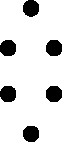
\includegraphics[height=1em]{tikz/hexdot.pdf}\hspace{0.5ex}}}

\newcommand{\sigi}{S\hexdot{}I\hexdot{}G\hexdot{}I\hexdot{}}


\newcommand{\eachpageornament}{%
	
\begin{tikzpicture}[remember picture, overlay]
	\node[anchor=north, rotate=45] at (current page.north west){%
		\pgfornament[opacity=\cornerop, width=1.5\secheight]{6}};
	\node[anchor=north, rotate=-45] at (current page.north east){%
		\pgfornament[opacity=\cornerop, width=1.5\secheight]{6}};
	\node[anchor=north, rotate=135] at (current page.south west){%
		\pgfornament[opacity=\cornerop, width=1.5\secheight]{6}};
	\node[anchor=north, rotate=-135] at (current page.south east){%
		\pgfornament[opacity=\cornerop, width=1.5\secheight]{6}};
	\end{tikzpicture}
}

\begin{document}
	
	\newgeometry{margin=0.4in}
	\begin{titlepage}
		\centering
		\vspace*{\fill}
		{\bfseries\LARGE
			Eighty Aphorisms and Maxims\\
		}
		\vspace*{0.5in}
		
\includegraphics[]{tikz/pantacle.pdf}\\
		\vspace*{0.5in}
		{\bfseries
			Louis-Claude de Saint-Martin\\
			\emph{Le Philosophe Inconnu}
		}   
		\vspace*{\fill}
	\end{titlepage}
	\restoregeometry
	
	\pagenumbering{gobble}
	
	\blankpage

	\eachpageornament	
	\vspace*{\fill}
	
	\begin{center}
		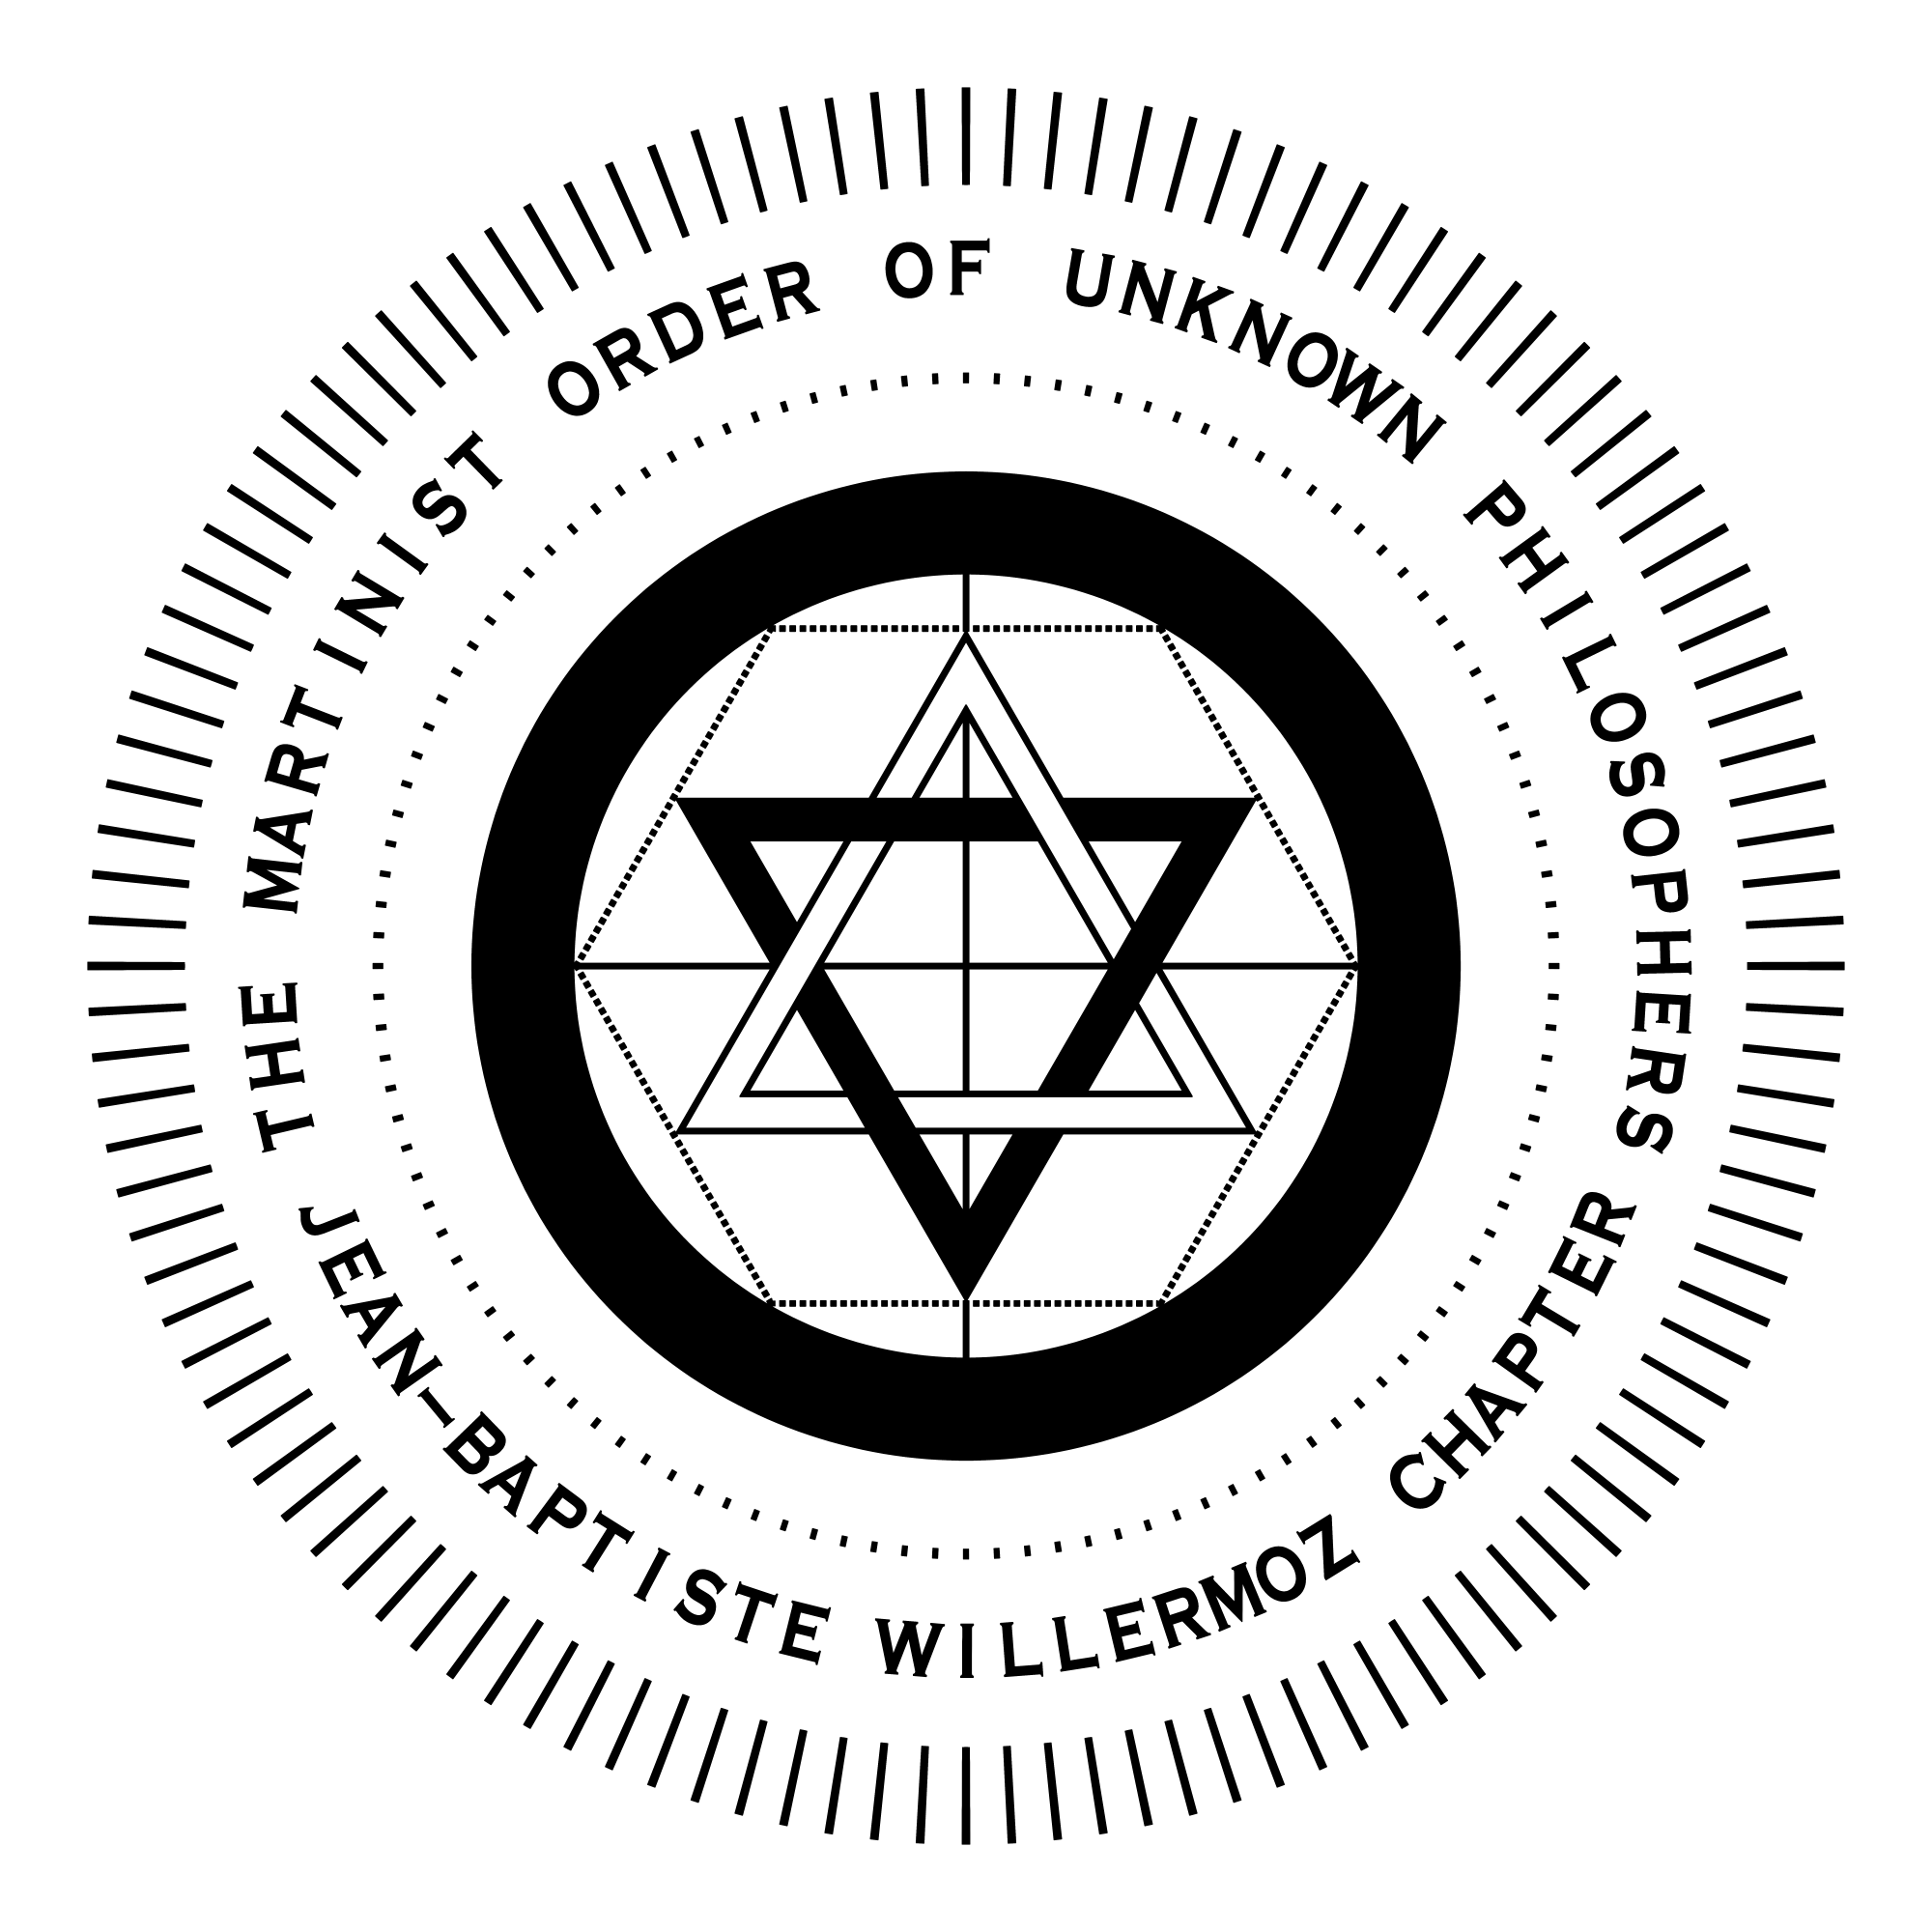
\includegraphics[width=\textwidth]{graphics/jbw_seal_2000px.png}\\\bigskip
		
		\textit{Published 2020}
	\end{center}
	
	\vspace*{\fill}
	
	\blankpage
	
	\eachpageornament
	\vspace*{\fill}
		
	This particular edition of \textit{Eighty Aphorisms and Maxims} was typeset and printed for use by the members of the Martinist Order of Unknown Philosophers, but all seekers of truth are encouraged to find wisdom in these pages.
	
	At time of publishing, the text of this book is the same as can be found in many places on the Internet, and no attempt has been made to edit or change it other than format it for printing, and to correct misspellings.
	
	To submit corrections to the text or format, or to ask us a question, please email: 
	
	\url{texanmartinist@gmail.com}
	
	\vspace*{\fill}
	
	\blankpage
	
	\eachpageornament
	\vspace*{\fill}
	
	\textit{This printing is dedicated to Grand Master Constant Martin Chevillon, \sigi{}, who was martyred for Truth, and to all of our Brothers and Sisters in Christ who have, do, or will suffer for their Faith.}
	
	\vspace*{\fill}
	
	\blankpage
	
	\aphorism{1}{God is all; the tongue of God is the spirit; the tongue of the spirit is science; the tongue of science should be the learned man. But the ordinary man of learning is like a signboard, and full too often of errors in orthography, like the signboards of small shops.}
	
	\aphorism{2}{Nature and the Scriptures should be compared. The priests misread the Scriptures: the philosophers misconstrue Nature. Hence they are always at war, and never compare their differences.}
	
	\aphorism{3}{When we speak of the Divine Sensibility, men tell us that God’s feelings are not as ours. But, this granted, it is for us to strive that we may feel like Him, without which we can in no wise become familiar with His operations, and still less be numbered among His servants. In truth, this Divine Sensibility is so absolutely the one thing needful, that apart therefrom, we are corpses, less even than stones, because stones abide in their law, and are that which they should be, whereas the soul of man was never designed to be a dead thing.}
	
	\aphorism{4}{There is nothing more easy than to come to the gate of truth; there is nothing more difficult than to enter it. This applies to most of the wise of this world.}
	
	\aphorism{5}{Great progress in truth is difficult in the midst of the world and under the favour of fortune; duplicity and double-seeming are needed in dealing with the one and anxiety for preserving the other. Our rest is not therefore in God.}
	
	\aphorism{6}{It is in vain that we pretend to arrive at the fullness of truth by reasoning. By this way we reach only rational truth; still it is infinitely precious, and full of resources against the assaults of false philosophy. The natural lights of every man of aspiration have indeed no other font, and it is therefore of almost universal use; but it cannot impart that sentiment and tact of active and radical truth from which our nature should derive its life and being. This kind of truth is given of itself alone. Let us make ourselves simple and childlike, and our faithful guide will cause us to feel its sweetness. If we profit by these first graces, we shall taste very soon those of the pure spirit, afterwards those of the Holy Spirit, then those of the Supreme Sanctity, and, lastly, in the interior man we shall behold the all.}
	
	\aphorism{7}{The sole advantage which can be found in the merits and joys of this world is that they cannot prevent us from dying.}
	
	\aphorism{8}{It is easy to understand why wisdom is a folly in the eyes of the world; it is because it shows by our own experience that the world is a folly by its side; for where is there a seeker after truth, however ardent, who has not delayed by the way, and has afterwards regarded himself as a fool when he has resumed the path of wisdom?}
	
	\aphorism{9}{If this world will seem to us, after our death, as nothing but magical illusion, why do we regard it otherwise at present? The nature of things does not change.}
	
	\aphorism{10}{Were I far from one loved and cherished, and did she send me her picture to sweeten the bitterness of absence, I should have certainly a kind of consolation, but I should not have a true joy. So has truth acted in regard to us. After our separation from her, she has bequeathed us her portrait, and this is the physical world, which she has placed before us to alleviate the misery of our privation. But what is the contemplation of the copy compared with that of the original?}
	
	\aphorism{11}{``All is vanity,'' says Solomon; but let courage, charity, and virtue be excluded from this teaching; rather, let us raise ourselves towards these sublime things, until we are able to say that all is truth, that all is love, that all is felicity.}
	
	\aphorism{12}{The learned describe nature;\\the wise explain it.}
	
	\aphorism{13}{Never persuade yourself that you possess wisdom in virtue of mere memory or mere mental culture. Wisdom is like a mother’s love, which makes itself felt only after the labours and pains of childbirth.}
	
	\aphorism{14}{Whatsoever is not wisdom only debauches man. With her he is fitted for all things, for the sentiments of nature, for lawful pleasures, for every virtue; in her absence the heart is petrified.}
	
	\aphorism{15}{It should be regarded as a grace of God when we are stripped successively of all human supports and succours, on which we are always too ready to depend. Thereby He compels us to repose only on Him, and herein is the final and most profound secret of wisdom. How can we be dejected at learning it?}
	
	\aphorism{16}{Had we the courage to make voluntarily the sincere and continual sacrifice of our entire being, the ordeals, oppositions, and evils which we undergo during life would not be sent us; hence we should always be superior to our sacrifices, like the Repairer, instead of being almost invariably inferior to them.}
	
	\aphorism{17}{As our material existence is not life, so our material destruction is not death.}
	
	\aphorism{18}{Death is the target at which all men strike; but the angle of incidence being equal to the angle of reflection, they find themselves after death in their former degree, whether above or below.}
	
	\aphorism{19}{Fear walks with those who dwell upon death, but those who think of life have love for their companion.}
	
	\aphorism{20}{Death should be regarded only as a relay in our journey; we reach it with exhausted horses, and we pause to get fresh ones able to carry us farther. But we must also pay what is due for the stage, already travelled, and until the account is settled, we are not allowed to go forward.}
	
	\aphorism{21}{The head of old was subject to the ruling of the heart, and served only to enlarge it. Today the scepter which belongs of right to the heart of man has been transferred to the head, which reigns in place of the heart. Love is more than knowledge, which is only the lamp of love, and the lamp is less than that which it enlightens.}
	
	\aphorism{22}{The man who believes in God can never fall into despair; the man who loves God must sigh incessantly.}
	
	\aphorism{23}{Love is the helm of our vessel; the sciences are only the weathercock on the capstan. A vessel can sail without a weathercock, but not without a helm.}
	
	\aphorism{24}{Science separates man from his fellows by creating distinctions with which prudence often forbids him to dispense. Love, on the contrary, impels men to communicate, and would establish everywhere the reign of that unity which is the principle from which it derives. The Repairer spoke nothing of the sciences, for he came not to divide men; he spoke only of love and the virtues, for he wished them to walk in unison. But science does not divide merely, it tends also to pride; love, on the other hand, does more than join together, it keeps man in humility. Hence St. Paul said that knowledge puffs up, but charity edifies.}
	
	\aphorism{25}{Science is for things of time, love for divine things. It is possible to dispense with science, but not with love, and by love will all be fulfilled, for thereby all began, and thereby does all exist. I would that all the teachings of the doctors of wisdom began and ended with these words: Love God, and you shall be learned as all the sages.}
	
	\aphorism{26}{For our personal advancement in virtue and truth one quality is sufficient, namely, love; to advance our fellows there must be two, love and intelligence; to accomplish the work of man there must be three love, intelligence, and activity. But love is ever the base and the fount in chief.}
	
	\aphorism{27}{Hope is faith beginning; faith is hope fulfilled; love is the living and visible operation of hope and faith.}
	
	\aphorism{28}{For most men life is made up of two days; in the first they believe everything, and in the second nothing. For some others life also has two days, but what distinguishes them from ordinary men is that in the first they believe only in illusions, and these are nothing; while in the second they believe in everything, for they believe in truth, which is all.}
	
	\aphorism{29}{The Gospel sufficiently impresses on us that the reward of many is with them in this world, whence they have little to expect in the other. This sentence, which, although severe, seems neither cruel nor unjust, has several degrees which it is well not to confound. There are men who will have received their entire recompense here below, others the half only, and yet others a fourth part. Thus the measure of compensations obtained in the present life will regulate the giving or refusing of those in the other. After this the expectations of the rich and happy on earth may be inferred easily.}
	
	\aphorism{30}{When deliverance has been accomplished, time is still required for self-correction and self-purification. In ceasing to be damned one is not therefore saved, and this is why there are two judgments in the Apocalypse.}
	
	\aphorism{31}{Believe not that the joys of the soul are a chimera, and that the goods we acquire in this life are lost utterly. The soul in no way changes its nature by leaving this mortal body. If given over to evil, it receives the punishment thereof by sinking further therein. But if it have loved goodness, and have at times experienced the secret delights of virtue, it will partake of them with increasing rapture. It has known here below the ravishments caused by the contemplation of things which transcend it. It seems as if nothing on earth can afford it like felicity; it seems even as if earthly pleasures had no existence. It may rely upon the same transports in the superior region; yet more, it may count upon joys beyond measure and uninterrupted delights when this gross material part shall no longer soil its purity. If it be thus, let us by no means neglect life; the greater our care for the soul here, the better shall be our estate hereafter.}
	
	\aphorism{32}{The law of spirit and of fire is to go up; the law of matter and of bodies is to go down. Hence, from the first moment of their existence, corporeal beings and beings corporised materially tend to their end and reintegration, each in their class.}
	
	\aphorism{33}{The locality of the soul has been a subject of frequent dispute; by some it has been placed in the head, by others in the heart, by yet others in the solar plexus. Were the soul an organic and material particle, there would be reason in assigning a place for it, as it would be possible that it should occupy one. But if it be a metaphysical entity, how can it be localized physically? Its faculties alone would seem to possess a determined seat --– the head for the functions of thought, meditation, judgment, and the heart for affections and sentiments of every kind. As for the soul itself, since its nature transcends both time and space, its correspondences and abode in space escape calculation.}
	
	\aphorism{34}{God is a fixed paradise, man should be a paradise in motion.}
	
	\aphorism{35}{Peace is found more often in patience than in judgment; hence it is better that we should be accused unjustly than that we should accuse others, even with justice.}
	
	\aphorism{36}{The Holy One quitted that which was above that He might come and restore us to life; we are reluctant to leave that which is below that we may recover the life which He has brought to us.}
	
	\aphorism{37}{Work for the spirit before asking the food of the spirit; he who will not work, let him not live.}
	
	\aphorism{38}{The greatest sin which we can commit against God is to doubt His love and mercy, for it is questioning the universality of His power, which is the persistent sin of the prince of darkness.}
	
	\aphorism{39}{The most sweet of our joys is to feel that God can wed with wisdom in us, or rather that without Him wisdom can never enter us, nor He without wisdom.}
	
	\aphorism{40}{All men who are instructed in fundamental truths speak the same language, for they are inhabitants of the same country.}
	
	\aphorism{41}{Men neglect habitually to study principles; and hence, when they have need to consider the development and functions of principles, they are astonished that they fail to understand them. But they believe themselves to have provided for everything by creating the word ``mystery.''}
	
	\aphorism{42}{Man’s head is raised towards heaven, and for this reason he finds nowhere to repose it on earth.}
	
	\aphorism{43}{All the goods of fortune are given us only to defray our journey through this earthly vale. But those who do not possess pass through it all the same, and this is infinitely consoling for the poor.}
	
	\aphorism{44}{The keynote of Nature is reluctance. Her unvaried occupation seems to be the withdrawal of her productions. She withdraws them even with violence to teach us that violence gave birth to them.}
	
	\aphorism{45}{Who is the innocent man? He who has acquired all things and has lost nothing.}
	
	\aphorism{46}{Preserve through all things the desire of the concupiscence of God; strive for its attainment, to overcome the illusion which surrounds us, and to realize our misery. Strive above all things to keep through all things the idea of the efficacious presence of a faithful friend who accompanies, guides, nourishes, and sustains us at every step. This will make us at once reserved and confident; it will give us both wisdom and strength. What would be wanting unto us if we were imbued invariably with these two virtues?}
	
	\aphorism{47}{We see that the earth, the stars, and all the wonders of Nature operate with exactitude and following a divine order; yet are we greater than these. 0 man! respect thyself, but fear to be unwise!}
	
	\aphorism{48}{The more we advance in virtue the less we perceive the defects of others, as a man on the summit of a mountain, with a vast prospect about him, beholds not the deformities of those who may dwell on the plain below. His very elevation should give him a lively and tender interest in those who, although beneath him, are, he knows, of his own nature. What then must be the love of God for men!}
	
	\aphorism{49}{All the impressions which are made on us by Nature are designed to exercise our soul during its term of penitence, to prompt us towards the eternal truths shown beneath a veil, and to lead us to recover what we have lost.}
	
	\aphorism{50}{The ordeals and oppositions which we undergo become our crosses when we remain beneath them, but they become ladders of ascent when we rise above them, and the wisdom which makes us their subject has no other end than our elevation and healing, and not that cruel and vengeful intent which is commonly attributed to it by the vulgar.}
	
	\aphorism{51}{It is insufficient to say unto God, ``Thy will be done;'' we must seek always to know that will; for if we know it not, who are we that we should accomplish it?}
	
	\aphorism{52}{The true method of expiating our faults is to repair them, and as regards those which are irreparable, not to be discouraged on account of them.}
	
	\aphorism{53}{We are all in a widowed state, and our task is to re-marry.}
	
	\aphorism{54}{Purification is accomplished only by union with the true law of our being; all who are outside that law can expiate nothing; they only contaminate themselves more deeply.}
	
	\aphorism{55}{That which is true is made by men subservient to the worship of the semblance, whereas the semblance was given them to be subservient to the worship of the true.}
	
	\aphorism{56}{There are for man three desirable things: \begin{enumerate}\item Never to forget that there is another light than the elementary, of which this is but the veil and the mask. \item To realise that nothing either can or should prevent him from accomplishing his work. \item To learn that what he knows best is that he knows nothing.\end{enumerate}}
	
	\aphorism{57}{The spirit is to our soul what our eyes are to our body; without it we should be nothing, even as apart from the life of the body the eyes are useless.}
	
	\aphorism{58}{Order thyself aright; that will instruct thee in wisdom and morality better than all the books which treat of them, for wisdom and morality are active forces.}
	
	\aphorism{59}{As a proof that we are regenerated we must regenerate everything around us.}
	
	\aphorism{60}{The wise of this world talk incessantly, and that upon all things false. The sages do not talk, but, like wisdom itself, they accomplish unceasingly the living and the true.}
	
	\aphorism{61}{The Church should be the Priest, but the Priest seeks to be the Church.}
	
	\aphorism{62}{Men of this world consider that it is impossible to be a saint without also being a fool. They do not know that, on the contrary, the one way to avoid being a fool is to be a saint.}
	
	\aphorism{63}{Mind and not soul is required for human sciences; but for real and divine sciences mind is not needed, for they are the offspring of the soul. Hence no two things can be more opposite than truth and the world.}
	
	\aphorism{64}{A picture without a frame is offensive in the eyes of the world, so accustomed is it to see frames without pictures.}
	
	\aphorism{65}{Unity is seldom found in associations; it must be sought in an individual junction with God. Only when that has been accomplished do we find brethren in one another.}
	
	\aphorism{66}{Words are given to us in trust, as sheep to a shepherd. If we leave them to go astray, to become famished, or to be devoured by wolves, we shall be called to a stricter account than he is.}
	
	\aphorism{67}{In order to demonstrate that the principle of any action is lawful, its consequences must be considered; where the actor is unhappy he is infallibly guilty, because he cannot be happy unless he is free.}
	
	\aphorism{68}{Whatsoever is sensible is relative, and there is nothing fixed therein.}
	
	\aphorism{69}{Man is one of the arbiters of God, and hence he is ancient as God, though there is not a plurality of Gods on this account.}
	
	\aphorism{70}{The kingdom of God is a continuous and complete activity. God is not the God of the dead, but of the living.}
	
	\aphorism{71}{If man avoids regarding himself as the king of the universe, it is because he lacks courage to recover his titles thereto, because its duties seem too laborious, and because he fears less to renounce his state and his rights than to undertake the restoration of their value.}
	
	\aphorism{72}{We are nearer to that which is not than to that which is.}
	
	\aphorism{73}{The prayer of the Spaniard, ``My God, defend me from myself,'' connects with a salutary feeling when we can awaken it within us, namely, that we ourselves are the only beings of whom we need be afraid on earth, whilst God is the one nature who has reason to fear only that which is not Himself. We might extend it as follows, '' My God, aid me in Thy goodness, that I may be spared from destroying thee.''}
	
	\aphorism{74}{If man, despite his state of reprobation, can still discern within himself a principle which is superior to his sensible and corporeal part, why should not such a principle be acknowledged in the sensible universe, equally distinct and superior, though deputed specially to govern it?}
	
	\aphorism{75}{I leave the unenlightened and shallow man to murmur at that justice which visits the trespasses of the parent upon his posterity. I will not even point to that physical law whereby an impure source communicates its impurities to its productions, because the analogy would be false and invidious if applied to what is not physical. But if justice can afflict the children through the fathers, it can also purify the fathers by the children; and though it exceeds the understanding of the ignorant, this should warrant us in suspending our judgment till we are admitted to the councils of wisdom.}
	
	\aphorism{76}{The thought of man is expressed in the material world, that of God in the universe.}
	
	\aphorism{77}{Sensible objects can give us nothing, but can deprive us of all. Our task while they encompass us is less to acquire than to lose nothing.}
	
	\aphorism{78}{The prayers and the truths which are taught us here below are too narrow for our needs; they are the prayers and the truths of time, and we feel that we were made for others.}
	
	\aphorism{79}{The universe is even as a great temple; the stars are its lights, the earth is its altar, all corporeal beings are its holocausts, and man, the priest of the Eternal, offers the sacrifices.}
	
	\aphorism{80}{The universe is also as a great fire lighted since the beginning of things for the purification of all corrupted beings.}
	
	\blankpage
	
	\vspace*{\fill}
	
	\begin{center}
		The Martinist Order\\of\\Unknown Philosophers\\\bigskip
		
		\url{http://www.moup.org/}
		
		\vspace*{\fill}
		
		This printing was produced on behalf of:\\\textit{Jean-Baptiste Willermoz Chapter}\\College Station, Texas.
		
		\vspace*{\fill}
		
		To submit questions or corrections:\\
		\url{texanmartinist@gmail.com}
	\end{center}
	
	\vspace*{\fill}
		
	\end{document}